\documentclass[12pt,a4paper]{article}

% ============================================================
% PAQUETES
% ============================================================
\usepackage[utf8]{inputenc}
\usepackage[T1]{fontenc}
\usepackage[spanish,mexico]{babel}
\usepackage{geometry}
\usepackage{graphicx}
\usepackage[table]{xcolor}
\usepackage{colortbl}
\usepackage{tabularx}
\usepackage{enumitem}
\usepackage{booktabs}
\usepackage{longtable}
\usepackage{array}
\usepackage{hyperref}
\usepackage{fancyhdr}
\usepackage{titlesec}
\usepackage{setspace}
\usepackage{needspace}

% ============================================================
% CONFIGURACIÓN DE PÁGINA
% ============================================================
\geometry{margin=2.5cm}
\setlength{\headheight}{14pt}
\setstretch{1.3}

% Colores de AbejaNet
\definecolor{abeja-primary}{RGB}{255, 193, 7}
\definecolor{abeja-dark}{RGB}{30, 30, 30}
\definecolor{abeja-text}{RGB}{51, 51, 51}

% Colores para fichas de requerimiento (estilo formato cliente)
\definecolor{secVerde}{RGB}{157, 186, 70}
\definecolor{cellGris}{RGB}{245, 245, 245}

% Comando para encabezado verde de sección dentro de la ficha
\newcommand{\secHeader}[2]{%
  \rowcolor{secVerde}\multicolumn{#1}{|l|}{\color{white}\textbf{#2}}\\\hline
}

% ============================================================
% HIPERENLACES
% ============================================================
\hypersetup{
  colorlinks=true,
  linkcolor=abeja-dark,
  urlcolor=abeja-primary,
  pdftitle={Requerimientos de la Aplicación Móvil — AbejaNet (Prototipo v3)},
  pdfauthor={Marco Antonio Gómez Olvera},
}

% ============================================================
% ENCABEZADO Y PIE
% ============================================================
\pagestyle{fancy}
\fancyhf{}
\fancyhead[L]{\small\textit{AbejaNet — Req. App Móvil (v3)}}
\fancyhead[R]{\small\textit{Adm. Proyectos de TI — IDGS 16}}
\fancyfoot[C]{\thepage}
\renewcommand{\headrulewidth}{0.4pt}

% ============================================================
% FORMATO DE TÍTULOS
% ============================================================
\titleformat{\section}{\Large\bfseries\color{abeja-dark}}{\thesection}{1em}{}
\titleformat{\subsection}{\large\bfseries\color{abeja-dark}}{\thesubsection}{1em}{}
\titleformat{\subsubsection}{\normalsize\bfseries\color{abeja-dark}}{\thesubsubsection}{1em}{}

% ============================================================
% INICIO DEL DOCUMENTO
% ============================================================
\begin{document}

% ---------------- Portada ----------------
\begin{titlepage}
  \begin{spacing}{1}
  \centering
  \vspace*{0.2cm}

  
\includegraphics[width=3.8cm]{images/logo_uteq.png}\\[0.3cm]

  {\LARGE\bfseries Especificación de Requerimientos}\\[0.2cm]
  {\Large\color{abeja-primary}\bfseries AbejaNet — Aplicación Móvil}\\[0.15cm]
  {\large\bfseries Prototipo Versión 3}\\[0.6cm]

  \rule{\textwidth}{1.5pt}\\[0.4cm]

  {\large\textbf{Materia:}}\\Administración de Proyectos de TI\\[0.1cm]
  {\large\textbf{Carrera:}}\\ Ingeniería en Desarrollo y Gestión de Software\\[0.1cm]
  {\large\textbf{Grupo:}}\\ IDGS 16\\[0.1cm]
  {\large\textbf{Periodo:}}\\ Mayo — Agosto 2026\\[0.1cm]
  {\large\textbf{Profesora:}}\\ Angélica Garduño Bustamante\\[0.3cm]

  \rule{\textwidth}{1.5pt}\\[0.3cm]

  {\large\textbf{Equipo de Trabajo}}\\[0.15cm]
  \begin{tabular}{ll}
    \textbf{Marco Antonio Gómez Olvera} & Programador de la Aplicación Móvil \\
    \textbf{Israel Gómez Bonilla} & Desarrollador de la Aplicación Web (Administrador) \\
    \textbf{Orlando Cabrera Rubio} & Encargado de IoT \\
    \textbf{Sandra Zoé Cabrera Velázquez} & Encargada de Documentación \\
  \end{tabular}\\[0.4cm]

  \rule{\textwidth}{1.5pt}\\[0.4cm]

  {\large\textbf{Unidad Tecnológica de Querétaro (UTEQ)}}\\[0.15cm]
  {\normalsize Querétaro, 5 de junio de 2026}

  \vfill
  \end{spacing}
\end{titlepage}

% ---------------- Índice ----------------
\tableofcontents
\newpage

% ---------------- SECCIONES ----------------
\section{Introducción}

\subsection{Contexto}

AbejaNet es una plataforma de monitoreo IoT para la apicultura que integra sensores ESP32, un backend en Node.js/PostgreSQL desplegado en Render, una aplicación web de administración y una aplicación móvil construida con React Native y Expo. La aplicación móvil permite a los apicultores supervisar en tiempo real la temperatura, humedad, peso y sonido de sus colmenas, así como recibir alertas críticas mediante notificaciones push.

El proyecto es desarrollado por un equipo multidisciplinario: \textbf{Marco Antonio Gómez Olvera} (programador de la aplicación móvil), \textbf{Israel Gómez Bonilla} (desarrollador de la aplicación web de administración), \textbf{Orlando Cabrera Rubio} (encargado de IoT) y \textbf{Sandra Zoé Cabrera Velázquez} (encargada de documentación).

Actualmente la aplicación cuenta con funcionalidades base implementadas: autenticación con JWT y refresh tokens, autenticación biométrica al reabrir la app, soporte de tema claro/oscuro, registro de usuarios con validación de contraseña fuerte, recuperación de contraseña por código de verificación, dashboard con resumen de apiarios, gestión de colmenas, alertas históricas y exportación de datos a CSV.

\subsection{Motivación de las Mejoras}

A partir de un análisis del código fuente y de la experiencia de uso, se identificaron áreas concretas en las que la aplicación puede elevar su calidad sin comprometer la estabilidad existente. Estas mejoras se concentran en tres ejes:

\begin{itemize}[leftmargin=*]
  \item \textbf{Experiencia de usuario (UX):} retroalimentación inmediata en formularios, internacionalización completa, retroalimentación háptica y notificaciones tipo \textit{toast} no intrusivas.
  \item \textbf{Seguridad:} prevención de envíos múltiples de peticiones (anti-spam), bloqueo automático por inactividad y resiliencia ante caídas de conexión.
  \item \textbf{Plus funcional:} una bitácora apícola digital con calendario que sustituye los cuadernos físicos tradicionales del apicultor.
\end{itemize}

\subsection{Objetivo del Documento}

El presente documento especifica \textbf{únicamente los requerimientos de la aplicación móvil} de AbejaNet correspondientes al \textbf{Prototipo Versión 3}. Quedan fuera de su alcance los requerimientos de la aplicación web de administración, del backend (salvo el soporte mínimo necesario para una funcionalidad móvil) y del subsistema IoT, los cuales se documentan por separado.

El documento se organiza en dos bloques: \textbf{requerimientos funcionales} y \textbf{requerimientos no funcionales}. Cada requerimiento es alcanzable dentro del cuatrimestre Mayo — Agosto 2026 y los requerimientos funcionales se complementan con un diagrama de casos de uso al final del documento.

\clearpage
\section{Alcance}

\subsection{Dentro del Alcance}

\begin{itemize}[leftmargin=*]
  \item Implementación en la aplicación móvil React Native (Expo SDK 51) del proyecto AbejaNet.
  \item Modificaciones puntuales al backend (Node.js / Express / PostgreSQL) únicamente para dar soporte a la bitácora apícola (RQF-05), funcionalidad propia de la app móvil.
  \item Internacionalización completa de las cadenas de texto que aún se encuentran codificadas en español dentro del frontend.
  \item Integración de las librerías \texttt{react-native-toast-message}, \texttt{@react-native-community/netinfo} y \texttt{react-native-calendars}.
  \item Reutilización del sistema de autenticación biométrica ya existente para el nuevo bloqueo por inactividad.
\end{itemize}

\subsection{Fuera del Alcance}

\begin{itemize}[leftmargin=*]
  \item Rediseño visual integral de pantallas ya existentes.
  \item Cambios de modelo de negocio o de roles de usuario.
  \item Integración con servicios externos de pago, mapas o análisis avanzado mediante inteligencia artificial.
  \item Modificaciones al firmware del ESP32 ni al protocolo de envío de lecturas.
  \item Requerimientos de la aplicación web de administración, del subsistema IoT (ESP32) o del backend que no estén directamente ligados a una funcionalidad de la app móvil; éstos se documentan por separado.
  \item Soporte para dispositivos wearables o Smart TV.
\end{itemize}

\subsection{Supuestos}

\begin{itemize}[leftmargin=*]
  \item El backend continuará desplegado en Render con la misma URL de producción.
  \item Los dispositivos de prueba contarán con Android 8.0 (API 26) o superior, o iOS 13.0 o superior.
  \item Los usuarios cuentan con conexión intermitente a internet; la app debe degradar correctamente cuando esta falle.
  \item Los apicultores que usen la bitácora tienen al menos una colmena registrada en el sistema.
\end{itemize}

\clearpage
\section{Control de Cambios}

\renewcommand{\arraystretch}{1.3}
\begin{flushright}
\begin{tabular}{|>{\columncolor{secVerde}}c|>{\columncolor{secVerde}}c|}
\hline
\textcolor{white}{\textbf{Edición}} & \textcolor{white}{\textbf{Fecha de Última Edición}} \\
\hline
\rowcolor{white}3 & 04/06/2026 \\
\hline
\end{tabular}
\end{flushright}

\vspace{0.4cm}

\begin{center}
\begin{tabular}{|c|p{4.5cm}|p{3.6cm}|p{2.8cm}|c|}
\hline
\rowcolor{secVerde}
\textcolor{white}{\textbf{Versión}} & \textcolor{white}{\textbf{Descripción del Cambio}} & \textcolor{white}{\textbf{Autor de Cambio}} & \textcolor{white}{\textbf{Rol}} & \textcolor{white}{\textbf{Fecha}} \\
\hline
1.0.0 & Creación del documento de requerimientos de la aplicación móvil (Prototipo v3). & Marco Antonio Gómez Olvera & Autor / Programador App Móvil & 01/06/2026 \\
\hline
1.0.1 & Revisión y estandarización documental del formato. & Sandra Zoé Cabrera Velázquez & Revisora / Encargada de Documentación & 03/06/2026 \\
\hline
1.0.2 & Aprobación final del documento para entrega. & Angélica Garduño Bustamante & Docente / Aprobadora & 04/06/2026 \\
\hline
\end{tabular}
\end{center}

\vspace{0.5cm}

Este documento especifica los ocho requerimientos de la aplicación móvil AbejaNet correspondientes al Prototipo Versión 3, agrupados en \textbf{requerimientos funcionales} (tres) y \textbf{requerimientos no funcionales} (cinco). Cada ficha contiene la información del cliente, la información general del requerimiento, su descripción detallada y las condiciones de prueba.

% ============================================================
% Requerimientos Funcionales
% ============================================================
\clearpage
\section{Requerimientos Funcionales}

Los requerimientos funcionales describen las capacidades y comportamientos concretos que la aplicación móvil debe ofrecer al usuario. La numeración continúa a partir de los requerimientos RQF-01 y RQF-02, ya implementados en prototipos anteriores (requerimiento general móvil y registro de clientes, respectivamente).

\clearpage
\subsection{RQF-03 — Anti-spam y validación de email}

\renewcommand{\arraystretch}{1.3}

% --- 1. Información del Cliente ---
\noindent
\begin{tabular}{|p{5cm}|p{10.5cm}|}
\hline
\rowcolor{secVerde}\multicolumn{2}{|l|}{\color{white}\textbf{1. INFORMACIÓN DEL CLIENTE}} \\
\hline
Nombre de la empresa  & UTEQ \\
\hline
Nombre del Contacto   & Angélica Garduño Bustamante \\
\hline
Fecha de Elaboración  & 01/06/2026 \\
\hline
\end{tabular}

\vspace{0.3cm}

% --- 2. Información General ---
\noindent
\begin{tabular}{|p{5cm}|p{10.5cm}|}
\hline
\rowcolor{secVerde}\multicolumn{2}{|l|}{\color{white}\textbf{2. INFORMACIÓN GENERAL}} \\
\hline
Nombre del Requerimiento     & RQF 03. Anti-spam y validación de email \\
\hline
Tipo de Requerimiento        & Funcional \\
\hline
Fecha requerida de solución  & 30/06/2026 \\
\hline
Prioridad                    & Alta \\
\hline
\end{tabular}

\vspace{0.3cm}

% --- 3. Descripción del Requerimiento ---
\noindent
\begin{tabular}{|p{4.5cm}|p{11cm}|}
\hline
\rowcolor{secVerde}\multicolumn{2}{|l|}{\color{white}\textbf{3. DESCRIPCIÓN DEL REQUERIMIENTO}} \\
\hline
Objetivo del Requerimiento &
Implementar un mecanismo de validación de email mediante expresión regular y un sistema anti-spam que deshabilite los botones de los formularios durante las peticiones HTTP, evitando envíos duplicados al backend. \\
\hline
Beneficio esperado &
Reducción de la carga al servidor por peticiones duplicadas, mejora de la experiencia de captura de datos del usuario y prevención de errores de validación previos al envío. \\
\hline
Alcance &
- Aplicar validación de email en \textit{login}, \textit{register} y \textit{forgot-password}. \par
- Deshabilitar el botón de envío durante la petición HTTP. \par
- Mostrar borde rojo y mensaje inline en inputs inválidos. \par
- No modifica la lógica del backend. \\
\hline
Ubicación &
\url{https://github.com/MarkG777/AbejaNet} \\
\hline
Descripción de Usuarios y Responsables &
\textbf{Usuarios:} \par
\textbf{Usuario (Cliente):} interactúa con los formularios de autenticación de la app móvil. \par
\vspace{0.1cm}
\textbf{Responsables:} \par
\textbf{App Móvil (React Native):} ejecuta la validación local antes de enviar la petición. \par
\textbf{API Backend:} no requiere cambios; solo recibe peticiones bien formadas. \\
\hline
Descripción funcional &
1. El usuario ingresa al formulario de inicio de sesión, registro o recuperación de contraseña. \par
2. Al escribir el email, el sistema valida el formato en tiempo real con una expresión regular. \par
3. Si el formato es inválido, el input muestra borde rojo y mensaje inline; el botón permanece deshabilitado. \par
4. Cuando los datos son válidos y el usuario presiona el botón de envío, el botón se deshabilita inmediatamente y muestra un indicador de carga. \par
5. Mientras la petición está en curso, el formulario no acepta nuevas interacciones. \par
6. Al recibirse la respuesta del backend, el botón se reactiva y se muestra el resultado correspondiente. \\
\hline
Restricciones &
- La validación local no sustituye la validación del backend. \par
- Debe mantenerse la compatibilidad con el sistema de autenticación JWT existente. \\
\hline
Precedencias & RQF 02. Registro de clientes \\
\hline
Documentación requerida & Manuales de usuario actualizados con la nueva retroalimentación visual. \\
\hline
Observaciones &
Se reutiliza la librería de iconos \texttt{Ionicons} ya presente en el proyecto para los indicadores visuales. \\
\hline
\end{tabular}

\vspace{0.3cm}

% --- 4. Condiciones de Prueba ---
\noindent
\begin{tabular}{|p{5.1cm}|p{5.1cm}|p{5.1cm}|}
\hline
\rowcolor{secVerde}\multicolumn{3}{|l|}{\color{white}\textbf{4. CONDICIONES DE PRUEBA}} \\
\hline
\rowcolor{cellGris}\textbf{Condición} & \textbf{Validación} & \textbf{Resultado} \\
\hline
El usuario ingresa un email con formato inválido en la pantalla de inicio de sesión. &
El sistema debe detectar el formato incorrecto antes de enviar la petición y mostrar un mensaje inline. &
El input se marca con borde rojo y el botón de envío permanece deshabilitado. \\
\hline
El usuario presiona repetidamente el botón \textit{``Iniciar sesión''} mientras la petición está en curso. &
El sistema debe deshabilitar el botón al primer clic para evitar envíos duplicados. &
Únicamente se realiza una petición HTTP al backend, sin importar el número de clics. \\
\hline
\end{tabular}

\clearpage
\subsection{RQF-04 — Indicador de conexión y caché offline del dashboard}

\renewcommand{\arraystretch}{1.3}

\noindent
\begin{tabular}{|p{5cm}|p{10.5cm}|}
\hline
\rowcolor{secVerde}\multicolumn{2}{|l|}{\color{white}\textbf{1. INFORMACIÓN DEL CLIENTE}} \\
\hline
Nombre de la empresa  & UTEQ \\ \hline
Nombre del Contacto   & Angélica Garduño Bustamante \\ \hline
Fecha de Elaboración  & 01/06/2026 \\ \hline
\end{tabular}

\vspace{0.3cm}

\noindent
\begin{tabular}{|p{5cm}|p{10.5cm}|}
\hline
\rowcolor{secVerde}\multicolumn{2}{|l|}{\color{white}\textbf{2. INFORMACIÓN GENERAL}} \\
\hline
Nombre del Requerimiento     & RQF 04. Indicador de conexión y caché offline del dashboard \\ \hline
Tipo de Requerimiento        & Funcional \\ \hline
Fecha requerida de solución  & 15/07/2026 \\ \hline
Prioridad                    & Alta \\ \hline
\end{tabular}

\vspace{0.3cm}

\noindent
\begin{tabular}{|p{4.5cm}|p{11cm}|}
\hline
\rowcolor{secVerde}\multicolumn{2}{|l|}{\color{white}\textbf{3. DESCRIPCIÓN DEL REQUERIMIENTO}} \\
\hline
Objetivo del Requerimiento &
Implementar un sistema de detección de conectividad y caché local del dashboard que permita al usuario consultar los últimos datos disponibles cuando no exista conexión a internet, mostrando un indicador visual claro de su estado. \\
\hline
Beneficio esperado &
La aplicación se mantiene utilizable durante caídas de conexión o \textit{cold starts} del backend. El usuario obtiene información reciente sin pantallas de carga infinita y comprende el estado de la red en todo momento. \\
\hline
Alcance &
- Integrar la librería \texttt{@react-native-community/netinfo}. \par
- Mostrar un banner superior cuando no haya conexión. \par
- Cachear el último resumen del dashboard en \texttt{AsyncStorage}. \par
- Refrescar automáticamente al recuperar conexión. \\
\hline
Ubicación & \url{https://github.com/MarkG777/AbejaNet} \\ \hline
Descripción de Usuarios y Responsables &
\textbf{Usuarios:} \par
\textbf{Usuario (Cliente):} consulta el dashboard con o sin conexión a internet. \par
\vspace{0.1cm}
\textbf{Responsables:} \par
\textbf{App Móvil:} detecta el estado de la red y administra el caché. \par
\textbf{AsyncStorage:} persiste localmente el último resumen recibido. \par
\textbf{API Backend:} provee los datos cuando hay conexión disponible. \\
\hline
Descripción funcional &
1. Al abrir el dashboard, la app consulta el estado de la red mediante \texttt{NetInfo}. \par
2. Si hay conexión, se descargan los datos del backend y se almacenan en caché con marca de tiempo. \par
3. Si no hay conexión, se muestra un banner superior amarillo con el mensaje \textit{``Sin conexión''}. \par
4. La pantalla muestra los últimos datos cacheados con la leyenda \textit{``Actualizado hace X min''}. \par
5. Cuando la conexión se restablece, la app refresca automáticamente los datos. \par
6. El banner desaparece al confirmarse la reconexión. \\
\hline
Restricciones &
- El caché debe limitarse al último resumen del dashboard para evitar consumo excesivo de almacenamiento. \par
- La marca de tiempo debe persistirse junto con los datos. \\
\hline
Precedencias & RQF 01. Requerimiento general Móvil \\ \hline
Documentación requerida & Manual de usuario actualizado con la nueva sección de comportamiento offline. \\ \hline
Observaciones & Se reutiliza el sistema de \texttt{AsyncStorage} ya integrado en el proyecto para tokens de sesión. \\ \hline
\end{tabular}

\vspace{0.3cm}

\noindent
\begin{tabular}{|p{5.1cm}|p{5.1cm}|p{5.1cm}|}
\hline
\rowcolor{secVerde}\multicolumn{3}{|l|}{\color{white}\textbf{4. CONDICIONES DE PRUEBA}} \\
\hline
\rowcolor{cellGris}\textbf{Condición} & \textbf{Validación} & \textbf{Resultado} \\
\hline
El usuario activa el modo avión con la app abierta en el dashboard. &
La app debe detectar la pérdida de conexión y reaccionar visualmente. &
Aparece el banner \textit{``Sin conexión''} y se muestran los datos cacheados con marca de tiempo. \\
\hline
El usuario abre la app sin conexión por primera vez tras tener datos cacheados. &
La app debe cargar los datos desde \texttt{AsyncStorage} sin intentar petición HTTP. &
El dashboard se renderiza con los datos cacheados en menos de 2 segundos. \\
\hline
\end{tabular}

\clearpage
\subsection{RQF-05 — Bitácora apícola con calendario}

\renewcommand{\arraystretch}{1.3}

\noindent
\begin{tabular}{|p{5cm}|p{10.5cm}|}
\hline
\rowcolor{secVerde}\multicolumn{2}{|l|}{\color{white}\textbf{1. INFORMACIÓN DEL CLIENTE}} \\
\hline
Nombre de la empresa  & UTEQ \\ \hline
Nombre del Contacto   & Angélica Garduño Bustamante \\ \hline
Fecha de Elaboración  & 01/06/2026 \\ \hline
\end{tabular}

\vspace{0.3cm}

\noindent
\begin{tabular}{|p{5cm}|p{10.5cm}|}
\hline
\rowcolor{secVerde}\multicolumn{2}{|l|}{\color{white}\textbf{2. INFORMACIÓN GENERAL}} \\
\hline
Nombre del Requerimiento     & RQF 05. Bitácora apícola con calendario \\ \hline
Tipo de Requerimiento        & Funcional \\ \hline
Fecha requerida de solución  & 30/07/2026 \\ \hline
Prioridad                    & Alta \\ \hline
\end{tabular}

\vspace{0.3cm}

\noindent
\begin{tabular}{|p{4.5cm}|p{11cm}|}
\hline
\rowcolor{secVerde}\multicolumn{2}{|l|}{\color{white}\textbf{3. DESCRIPCIÓN DEL REQUERIMIENTO}} \\
\hline
Objetivo del Requerimiento &
Implementar una bitácora apícola digital con calendario interactivo que permita al apicultor registrar, consultar, editar y eliminar eventos asociados a sus colmenas y apiarios, sustituyendo la libreta de campo tradicional. \\
\hline
Beneficio esperado &
Centralización del historial de inspecciones, tratamientos, cosechas y cambios de reina en un solo lugar accesible desde el dispositivo móvil. Mejora la trazabilidad de las labores apícolas y facilita la toma de decisiones informadas. \\
\hline
Alcance &
- Crear nueva pantalla \textit{Bitácora} accesible desde el \textit{drawer} del usuario. \par
- Mostrar un calendario mensual con dots de color en los días con eventos. \par
- CRUD completo de eventos clasificados por tipo. \par
- Acceso rápido desde la pantalla de detalle de cada colmena. \par
- Crear tabla \texttt{bitacora} en PostgreSQL y endpoints REST asociados. \\
\hline
Ubicación & \url{https://github.com/MarkG777/AbejaNet} \\ \hline
Descripción de Usuarios y Responsables &
\textbf{Usuarios:} \par
\textbf{Apicultor (Cliente):} registra y consulta eventos sobre el manejo de sus colmenas. \par
\vspace{0.1cm}
\textbf{Responsables:} \par
\textbf{App Móvil:} ofrece la interfaz de calendario y los formularios de evento. \par
\textbf{API Backend:} expone los endpoints \texttt{/api/bitacora} para CRUD. \par
\textbf{Base de Datos PostgreSQL:} almacena los eventos en la tabla \texttt{bitacora} con relaciones a \texttt{usuarios}, \texttt{colmenas} y \texttt{apiarios}. \\
\hline
Descripción funcional &
1. El apicultor accede a \textit{Bitácora} desde el \textit{drawer} del usuario. \par
2. Visualiza un calendario mensual con dots de color en los días con eventos registrados. \par
3. Selecciona un día y consulta el listado de eventos de esa fecha. \par
4. Mediante un botón flotante (FAB) crea un nuevo evento eligiendo tipo (Inspección, Cosecha, Tratamiento, Cambio de reina, División/Unión, Alimentación o Nota libre), colmena/apiario asociado, título y comentario. \par
5. Puede editar o eliminar eventos existentes. \par
6. Desde la pantalla de detalle de una colmena, dispone de un acceso rápido \textit{``Registrar evento''} que pre-llena la colmena en el formulario. \par
7. Puede filtrar el calendario por colmena o apiario específico. \\
\hline
Restricciones &
- Cada evento debe estar asociado al menos a una colmena o a un apiario. \par
- Los comentarios libres tienen un límite de 1000 caracteres. \par
- Solo el usuario propietario puede ver y modificar sus propios eventos. \\
\hline
Precedencias & RQF 02. Registro de clientes \\ \hline
Documentación requerida & Manual de usuario con guía de uso de la bitácora y descripción de los tipos de evento. \\ \hline
Observaciones & Se introduce la librería \texttt{react-native-calendars} y se requiere actualización del esquema de base de datos. \\ \hline
\end{tabular}

\vspace{0.3cm}

\noindent
\begin{tabular}{|p{5.1cm}|p{5.1cm}|p{5.1cm}|}
\hline
\rowcolor{secVerde}\multicolumn{3}{|l|}{\color{white}\textbf{4. CONDICIONES DE PRUEBA}} \\
\hline
\rowcolor{cellGris}\textbf{Condición} & \textbf{Validación} & \textbf{Resultado} \\
\hline
El apicultor crea un nuevo evento de tipo \textit{Inspección} desde la pantalla de bitácora. &
El sistema debe persistir el evento en el backend y reflejarlo en el calendario. &
El día correspondiente muestra un dot de color y al seleccionarlo aparece el evento creado. \\
\hline
El apicultor accede a \textit{``Registrar evento''} desde el detalle de una colmena. &
El formulario debe abrirse con la colmena pre-seleccionada en el campo correspondiente. &
El evento se guarda asociado correctamente a esa colmena sin requerir selección manual. \\
\hline
\end{tabular}


% ============================================================
% Requerimientos No Funcionales
% ============================================================
\clearpage
\section{Requerimientos No Funcionales}

Los requerimientos no funcionales describen las cualidades transversales de la aplicación móvil (usabilidad, seguridad, portabilidad y rendimiento). Al no representar interacciones discretas del usuario, no se acompañan de diagramas de casos de uso.

\clearpage
\subsection{RNF-01 — Soporte bilingüe Español / Inglés}

\renewcommand{\arraystretch}{1.3}

\noindent
\begin{tabular}{|p{5cm}|p{10.5cm}|}
\hline
\rowcolor{secVerde}\multicolumn{2}{|l|}{\color{white}\textbf{1. INFORMACIÓN DEL CLIENTE}} \\
\hline
Nombre de la empresa  & UTEQ \\ \hline
Nombre del Contacto   & Angélica Garduño Bustamante \\ \hline
Fecha de Elaboración  & 01/06/2026 \\ \hline
\end{tabular}

\vspace{0.3cm}

\noindent
\begin{tabular}{|p{5cm}|p{10.5cm}|}
\hline
\rowcolor{secVerde}\multicolumn{2}{|l|}{\color{white}\textbf{2. INFORMACIÓN GENERAL}} \\
\hline
Nombre del Requerimiento     & RNF 01. Soporte bilingüe Español / Inglés \\ \hline
Tipo de Requerimiento        & No funcional — Usabilidad \\ \hline
Fecha requerida de solución  & 25/06/2026 \\ \hline
Prioridad                    & Media \\ \hline
\end{tabular}

\vspace{0.3cm}

\noindent
\begin{tabular}{|p{4.5cm}|p{11cm}|}
\hline
\rowcolor{secVerde}\multicolumn{2}{|l|}{\color{white}\textbf{3. DESCRIPCIÓN DEL REQUERIMIENTO}} \\
\hline
Objetivo del Requerimiento &
Garantizar que la totalidad de las cadenas de texto visibles para el usuario estén disponibles en español e inglés, permitiendo el cambio dinámico del idioma desde la pantalla de perfil. \\
\hline
Beneficio esperado &
Accesibilidad para usuarios anglófonos, experiencia profesional consistente y posibilidad de uso académico internacional del proyecto. \\
\hline
Alcance &
- Extraer las cadenas hardcoded restantes (\texttt{login}, \texttt{register}, \texttt{onboarding}, alertas) hacia los archivos \texttt{locales/es.json} y \texttt{locales/en.json}. \par
- Localizar el formato de fechas según el idioma activo. \par
- Persistir la preferencia de idioma en \texttt{AsyncStorage}. \\
\hline
Ubicación & \url{https://github.com/MarkG777/AbejaNet} \\ \hline
Descripción de Usuarios y Responsables &
\textbf{Usuarios:} \par
\textbf{Usuario (Cliente):} cambia el idioma desde el perfil. \par
\vspace{0.1cm}
\textbf{Responsables:} \par
\textbf{App Móvil:} aplica el idioma seleccionado a través de \texttt{react-i18next}. \par
\textbf{AsyncStorage:} persiste la preferencia entre sesiones. \\
\hline
Descripción funcional &
1. El usuario accede a su perfil y elige el idioma deseado. \par
2. Toda la interfaz se actualiza al instante sin reiniciar la app. \par
3. La preferencia se almacena localmente y se aplica al siguiente arranque. \par
4. Los formatos de fecha y hora se muestran según la convención del idioma activo. \\
\hline
Restricciones &
- Solo se soportan español e inglés en esta iteración. \par
- Las claves nuevas deben mantener consistencia entre ambos archivos JSON. \\
\hline
Precedencias & Ninguna (la base de \texttt{i18next} ya existe en el proyecto). \\ \hline
Documentación requerida & Manual técnico con la convención de claves de internacionalización. \\ \hline
Observaciones & La librería \texttt{react-i18next} ya se encuentra instalada en el proyecto. \\ \hline
\end{tabular}

\vspace{0.3cm}

\noindent
\begin{tabular}{|p{5.1cm}|p{5.1cm}|p{5.1cm}|}
\hline
\rowcolor{secVerde}\multicolumn{3}{|l|}{\color{white}\textbf{4. CONDICIONES DE PRUEBA}} \\
\hline
\rowcolor{cellGris}\textbf{Condición} & \textbf{Validación} & \textbf{Resultado} \\
\hline
El usuario cambia el idioma de español a inglés desde el perfil. &
La interfaz debe traducirse en tiempo real, incluyendo formularios, validaciones y alertas. &
Todos los textos visibles cambian al inglés sin reiniciar la app. \\
\hline
El usuario cierra y vuelve a abrir la app después de haber cambiado el idioma. &
La preferencia debe persistir entre sesiones. &
La app inicia automáticamente con el idioma previamente seleccionado. \\
\hline
\end{tabular}

\clearpage
\subsection{RNF-02 — Retroalimentación háptica y toasts no intrusivos}

\renewcommand{\arraystretch}{1.3}

\noindent
\begin{tabular}{|p{5cm}|p{10.5cm}|}
\hline
\rowcolor{secVerde}\multicolumn{2}{|l|}{\color{white}\textbf{1. INFORMACIÓN DEL CLIENTE}} \\
\hline
Nombre de la empresa  & UTEQ \\ \hline
Nombre del Contacto   & Angélica Garduño Bustamante \\ \hline
Fecha de Elaboración  & 01/06/2026 \\ \hline
\end{tabular}

\vspace{0.3cm}

\noindent
\begin{tabular}{|p{5cm}|p{10.5cm}|}
\hline
\rowcolor{secVerde}\multicolumn{2}{|l|}{\color{white}\textbf{2. INFORMACIÓN GENERAL}} \\
\hline
Nombre del Requerimiento     & RNF 02. Retroalimentación háptica y toasts no intrusivos \\ \hline
Tipo de Requerimiento        & No funcional — Usabilidad \\ \hline
Fecha requerida de solución  & 30/06/2026 \\ \hline
Prioridad                    & Media \\ \hline
\end{tabular}

\vspace{0.3cm}

\noindent
\begin{tabular}{|p{4.5cm}|p{11cm}|}
\hline
\rowcolor{secVerde}\multicolumn{2}{|l|}{\color{white}\textbf{3. DESCRIPCIÓN DEL REQUERIMIENTO}} \\
\hline
Objetivo del Requerimiento &
Sustituir las alertas modales (\texttt{Alert.alert}) por notificaciones tipo \textit{toast} no intrusivas y agregar retroalimentación háptica en las acciones críticas de la app. \\
\hline
Beneficio esperado &
La aplicación adquiere una sensación nativa y fluida, alineada con las mejores prácticas de apps móviles modernas. El usuario recibe confirmación de sus acciones sin interrupciones de flujo. \\
\hline
Alcance &
- Integrar la librería \texttt{react-native-toast-message}. \par
- Aprovechar \texttt{expo-haptics} (ya instalada) en login, guardado de perfil, registro de evento y marcado de alertas como leídas. \par
- Mantener \texttt{Alert.alert} solo para confirmaciones destructivas (eliminar cuenta, eliminar registros). \\
\hline
Ubicación & \url{https://github.com/MarkG777/AbejaNet} \\ \hline
Descripción de Usuarios y Responsables &
\textbf{Usuarios:} \par
\textbf{Usuario (Cliente):} ejecuta acciones que generan retroalimentación háptica y visual. \par
\vspace{0.1cm}
\textbf{Responsables:} \par
\textbf{App Móvil:} dispara la vibración y muestra los toasts en respuesta a las acciones del usuario. \\
\hline
Descripción funcional &
1. Cuando el usuario ejecuta una acción crítica, la app dispara una vibración suave mediante \texttt{expo-haptics}. \par
2. El resultado de la acción se muestra como toast (verde para éxito, rojo para error, amarillo para advertencia) en la parte inferior de la pantalla. \par
3. El toast desaparece automáticamente tras 3 segundos sin bloquear la interfaz. \par
4. Las acciones destructivas continúan mostrando confirmación modal previa. \\
\hline
Restricciones &
- La intensidad háptica debe ser \texttt{Light} para no resultar molesta. \par
- Los toasts no deben superponerse con la barra de navegación inferior. \\
\hline
Precedencias & Ninguna (las dependencias ya están en el proyecto). \\ \hline
Documentación requerida & No se requiere documentación adicional para el usuario final. \\ \hline
Observaciones & La librería \texttt{expo-haptics} ya es utilizada parcialmente en el componente \texttt{HapticTab}. \\ \hline
\end{tabular}

\vspace{0.3cm}

\noindent
\begin{tabular}{|p{5.1cm}|p{5.1cm}|p{5.1cm}|}
\hline
\rowcolor{secVerde}\multicolumn{3}{|l|}{\color{white}\textbf{4. CONDICIONES DE PRUEBA}} \\
\hline
\rowcolor{cellGris}\textbf{Condición} & \textbf{Validación} & \textbf{Resultado} \\
\hline
El usuario guarda cambios en su perfil correctamente. &
La app debe vibrar suavemente y mostrar un toast de éxito. &
Aparece un toast verde \textit{``Perfil actualizado''} y se siente la vibración háptica. \\
\hline
El usuario ingresa credenciales incorrectas en el inicio de sesión. &
La app debe mostrar un toast rojo en lugar de un \texttt{Alert.alert}. &
Aparece un toast rojo \textit{``Credenciales inválidas''} sin bloquear la pantalla de login. \\
\hline
\end{tabular}

\clearpage
\subsection{RNF-03 — Bloqueo automático por inactividad}

\renewcommand{\arraystretch}{1.3}

\noindent
\begin{tabular}{|p{5cm}|p{10.5cm}|}
\hline
\rowcolor{secVerde}\multicolumn{2}{|l|}{\color{white}\textbf{1. INFORMACIÓN DEL CLIENTE}} \\
\hline
Nombre de la empresa  & UTEQ \\ \hline
Nombre del Contacto   & Angélica Garduño Bustamante \\ \hline
Fecha de Elaboración  & 01/06/2026 \\ \hline
\end{tabular}

\vspace{0.3cm}

\noindent
\begin{tabular}{|p{5cm}|p{10.5cm}|}
\hline
\rowcolor{secVerde}\multicolumn{2}{|l|}{\color{white}\textbf{2. INFORMACIÓN GENERAL}} \\
\hline
Nombre del Requerimiento     & RNF 03. Bloqueo automático por inactividad \\ \hline
Tipo de Requerimiento        & No funcional — Seguridad \\ \hline
Fecha requerida de solución  & 20/07/2026 \\ \hline
Prioridad                    & Alta \\ \hline
\end{tabular}

\vspace{0.3cm}

\noindent
\begin{tabular}{|p{4.5cm}|p{11cm}|}
\hline
\rowcolor{secVerde}\multicolumn{2}{|l|}{\color{white}\textbf{3. DESCRIPCIÓN DEL REQUERIMIENTO}} \\
\hline
Objetivo del Requerimiento &
Bloquear automáticamente la aplicación tras un periodo de inactividad del usuario en primer plano, exigiendo autenticación biométrica para reanudar el uso y proteger la información sensible del apiario. \\
\hline
Beneficio esperado &
Capa adicional de seguridad sin requerir el reingreso constante de la contraseña. Protección de datos en escenarios donde el usuario deja el dispositivo desbloqueado por error. \\
\hline
Alcance &
- Implementar un temporizador global de inactividad con duración predeterminada de 5 minutos. \par
- Detectar interacciones del usuario mediante un \textit{wrapper} a nivel de aplicación. \par
- Reutilizar el sistema de \texttt{LocalAuthentication} ya existente para el bloqueo. \par
- Cerrar sesión tras tres intentos biométricos fallidos. \\
\hline
Ubicación & \url{https://github.com/MarkG777/AbejaNet} \\ \hline
Descripción de Usuarios y Responsables &
\textbf{Usuarios:} \par
\textbf{Usuario (Cliente):} reanuda el uso de la app tras un periodo de inactividad. \par
\vspace{0.1cm}
\textbf{Responsables:} \par
\textbf{App Móvil:} mide el tiempo de inactividad y dispara la pantalla biométrica. \par
\textbf{Sistema operativo:} provee la API de autenticación biométrica nativa. \\
\hline
Descripción funcional &
1. Mientras la app está en primer plano, un temporizador global mide el tiempo desde la última interacción del usuario. \par
2. Si transcurren 5 minutos sin interacción, se dispara la pantalla biométrica. \par
3. Si la autenticación es exitosa, el usuario regresa a la pantalla en la que estaba. \par
4. Si falla 3 veces, la sesión se cierra y se redirige a la pantalla de inicio de sesión. \par
5. Cualquier interacción (toque, scroll) reinicia el temporizador. \\
\hline
Restricciones &
- El temporizador se pausa cuando la app pasa a segundo plano (ya está cubierto por la biometría existente). \par
- El umbral de 5 minutos no es configurable por el usuario en esta iteración. \\
\hline
Precedencias & Sistema biométrico ya implementado en \texttt{AuthContext}. \\ \hline
Documentación requerida & Manual de usuario con sección sobre el bloqueo automático. \\ \hline
Observaciones & Reutiliza \texttt{expo-local-authentication} ya integrada en el proyecto. \\ \hline
\end{tabular}

\vspace{0.3cm}

\noindent
\begin{tabular}{|p{5.1cm}|p{5.1cm}|p{5.1cm}|}
\hline
\rowcolor{secVerde}\multicolumn{3}{|l|}{\color{white}\textbf{4. CONDICIONES DE PRUEBA}} \\
\hline
\rowcolor{cellGris}\textbf{Condición} & \textbf{Validación} & \textbf{Resultado} \\
\hline
El usuario deja la app abierta sin interacción por más de 5 minutos. &
El sistema debe disparar la pantalla biométrica de bloqueo. &
Aparece la solicitud de huella o Face ID; al validarse, el usuario regresa a la pantalla previa. \\
\hline
El usuario falla tres veces consecutivas la autenticación biométrica de bloqueo. &
El sistema debe cerrar la sesión por seguridad. &
La app cierra sesión y redirige al usuario a la pantalla de inicio de sesión. \\
\hline
\end{tabular}

\clearpage
\subsection{RNF-04 — Compatibilidad multiplataforma}

\renewcommand{\arraystretch}{1.3}

\noindent
\begin{tabular}{|p{5cm}|p{10.5cm}|}
\hline
\rowcolor{secVerde}\multicolumn{2}{|l|}{\color{white}\textbf{1. INFORMACIÓN DEL CLIENTE}} \\
\hline
Nombre de la empresa  & UTEQ \\ \hline
Nombre del Contacto   & Angélica Garduño Bustamante \\ \hline
Fecha de Elaboración  & 01/06/2026 \\ \hline
\end{tabular}

\vspace{0.3cm}

\noindent
\begin{tabular}{|p{5cm}|p{10.5cm}|}
\hline
\rowcolor{secVerde}\multicolumn{2}{|l|}{\color{white}\textbf{2. INFORMACIÓN GENERAL}} \\
\hline
Nombre del Requerimiento     & RNF 04. Compatibilidad multiplataforma \\ \hline
Tipo de Requerimiento        & No funcional — Portabilidad \\ \hline
Fecha requerida de solución  & 30/07/2026 \\ \hline
Prioridad                    & Media \\ \hline
\end{tabular}

\vspace{0.3cm}

\noindent
\begin{tabular}{|p{4.5cm}|p{11cm}|}
\hline
\rowcolor{secVerde}\multicolumn{2}{|l|}{\color{white}\textbf{3. DESCRIPCIÓN DEL REQUERIMIENTO}} \\
\hline
Objetivo del Requerimiento &
Garantizar que la aplicación móvil ejecute correctamente todas sus funcionalidades, incluidas las nuevas, en Android 8.0 (API 26) o superior y en iOS 13.0 o superior. \\
\hline
Beneficio esperado &
Cobertura de la mayoría de los dispositivos en uso por el público objetivo (apicultores) sin necesidad de hardware reciente. Reduce el riesgo de exclusión por incompatibilidad. \\
\hline
Alcance &
- Declarar las versiones mínimas en \texttt{app.json}. \par
- Validar las nuevas dependencias contra las versiones mínimas. \par
- Probar en al menos un emulador de Android 8 y un simulador de iOS 13. \\
\hline
Ubicación & \url{https://github.com/MarkG777/AbejaNet} \\ \hline
Descripción de Usuarios y Responsables &
\textbf{Usuarios:} \par
\textbf{Usuario (Cliente):} ejecuta la app desde un dispositivo móvil de gama media. \par
\vspace{0.1cm}
\textbf{Responsables:} \par
\textbf{Equipo de desarrollo:} configura las versiones mínimas y ejecuta pruebas en emuladores. \par
\textbf{Expo SDK 51:} provee la base de compatibilidad multiplataforma. \\
\hline
Descripción funcional &
1. La app debe instalarse y ejecutarse en Android 8.0 o superior. \par
2. La app debe instalarse y ejecutarse en iOS 13.0 o superior. \par
3. Todas las funcionalidades nuevas (RQF 03 a RQF 05) deben verificarse en ambos sistemas operativos. \par
4. Las versiones mínimas se documentan en \texttt{app.json} y en el \texttt{README}. \\
\hline
Restricciones &
- No se garantiza compatibilidad con Android $<$ 8.0 ni iOS $<$ 13.0. \par
- Las funciones biométricas dependen del hardware del dispositivo. \\
\hline
Precedencias & Ninguna. \\ \hline
Documentación requerida & \texttt{README} actualizado con las versiones mínimas. \\ \hline
Observaciones & Esta compatibilidad ya se garantiza por defecto al utilizar Expo SDK 51. \\ \hline
\end{tabular}

\vspace{0.3cm}

\noindent
\begin{tabular}{|p{5.1cm}|p{5.1cm}|p{5.1cm}|}
\hline
\rowcolor{secVerde}\multicolumn{3}{|l|}{\color{white}\textbf{4. CONDICIONES DE PRUEBA}} \\
\hline
\rowcolor{cellGris}\textbf{Condición} & \textbf{Validación} & \textbf{Resultado} \\
\hline
La app se instala en un emulador de Android 8.0 (API 26). &
Todas las pantallas y funcionalidades deben renderizarse sin errores. &
La app inicia correctamente y permite navegar por todas las pantallas. \\
\hline
La app se instala en un simulador de iOS 13.0. &
La biometría, las notificaciones y el almacenamiento seguro deben funcionar. &
Todas las funciones críticas operan sin advertencias de compatibilidad. \\
\hline
\end{tabular}

\clearpage
\subsection{RNF-05 — Tiempo de respuesta en operaciones locales}

\renewcommand{\arraystretch}{1.3}

\noindent
\begin{tabular}{|p{5cm}|p{10.5cm}|}
\hline
\rowcolor{secVerde}\multicolumn{2}{|l|}{\color{white}\textbf{1. INFORMACIÓN DEL CLIENTE}} \\
\hline
Nombre de la empresa  & UTEQ \\ \hline
Nombre del Contacto   & Angélica Garduño Bustamante \\ \hline
Fecha de Elaboración  & 01/06/2026 \\ \hline
\end{tabular}

\vspace{0.3cm}

\noindent
\begin{tabular}{|p{5cm}|p{10.5cm}|}
\hline
\rowcolor{secVerde}\multicolumn{2}{|l|}{\color{white}\textbf{2. INFORMACIÓN GENERAL}} \\
\hline
Nombre del Requerimiento     & RNF 05. Tiempo de respuesta en operaciones locales \\ \hline
Tipo de Requerimiento        & No funcional — Rendimiento \\ \hline
Fecha requerida de solución  & 30/07/2026 \\ \hline
Prioridad                    & Media \\ \hline
\end{tabular}

\vspace{0.3cm}

\noindent
\begin{tabular}{|p{4.5cm}|p{11cm}|}
\hline
\rowcolor{secVerde}\multicolumn{2}{|l|}{\color{white}\textbf{3. DESCRIPCIÓN DEL REQUERIMIENTO}} \\
\hline
Objetivo del Requerimiento &
Garantizar que las operaciones locales de la aplicación se completen en un tiempo máximo de dos (2) segundos en dispositivos de gama media, sin bloquear el hilo principal de la interfaz. \\
\hline
Beneficio esperado &
Sensación de fluidez y respuesta inmediata en las acciones del usuario, alineada con los estándares de apps móviles modernas. \\
\hline
Alcance &
- Cambio de pantalla mediante \textit{Expo Router}. \par
- Cambio de idioma desde el perfil. \par
- Apertura de la pantalla de bitácora. \par
- Validación de formularios. \par
- Lectura del caché del dashboard. \\
\hline
Ubicación & \url{https://github.com/MarkG777/AbejaNet} \\ \hline
Descripción de Usuarios y Responsables &
\textbf{Usuarios:} \par
\textbf{Usuario (Cliente):} percibe la fluidez de la aplicación. \par
\vspace{0.1cm}
\textbf{Responsables:} \par
\textbf{Equipo de desarrollo:} mide y documenta los tiempos de respuesta usando \texttt{performance.now()} en dispositivos de prueba. \\
\hline
Descripción funcional &
1. Las operaciones locales no deben exceder los 2 segundos en su ejecución. \par
2. Las operaciones que dependan de la red están exentas de este requerimiento. \par
3. Las animaciones deben ejecutarse a 60 FPS sin caídas perceptibles. \par
4. Los tiempos se documentan en una tabla del \texttt{README} técnico. \\
\hline
Restricciones &
- La métrica aplica solo a operaciones locales (sin red). \par
- Se considera \textit{gama media} a un dispositivo con al menos 4 GB de RAM. \\
\hline
Precedencias & Ninguna. \\ \hline
Documentación requerida & Tabla de tiempos medidos en el \texttt{README} técnico. \\ \hline
Observaciones & Las dependencias actuales (\texttt{react-native-reanimated}) ya facilitan el cumplimiento del requerimiento. \\ \hline
\end{tabular}

\vspace{0.3cm}

\noindent
\begin{tabular}{|p{5.1cm}|p{5.1cm}|p{5.1cm}|}
\hline
\rowcolor{secVerde}\multicolumn{3}{|l|}{\color{white}\textbf{4. CONDICIONES DE PRUEBA}} \\
\hline
\rowcolor{cellGris}\textbf{Condición} & \textbf{Validación} & \textbf{Resultado} \\
\hline
El usuario navega del dashboard a la pantalla de bitácora. &
La transición debe completarse en menos de 2 segundos. &
La pantalla de bitácora se renderiza con el calendario visible dentro del umbral establecido. \\
\hline
El usuario cambia el idioma desde el perfil. &
La interfaz debe actualizarse en tiempo real sin bloquear la UI. &
La traducción se aplica en menos de 1 segundo y la app responde inmediatamente a nuevas interacciones. \\
\hline
\end{tabular}


\clearpage
\section{Diagramas de Casos de Uso}
\label{sec:casos_uso}

A continuación se presentan los diagramas de casos de uso correspondientes a los tres requerimientos funcionales (RQF-03, RQF-04 y RQF-05) descritos en la sección de Requerimientos Funcionales. Los requerimientos no funcionales no se diagraman por tratarse de cualidades transversales del sistema y no de interacciones discretas del usuario.

\subsection{RQF-03 — Anti-spam y validación de email}

El siguiente diagrama describe la interacción del usuario con cualquiera de los formularios de autenticación (inicio de sesión, registro o recuperación de contraseña). La validación local previene el envío de peticiones HTTP con datos malformados y el bloqueo del botón impide envíos duplicados.

\begin{figure}[h!]
  \centering
  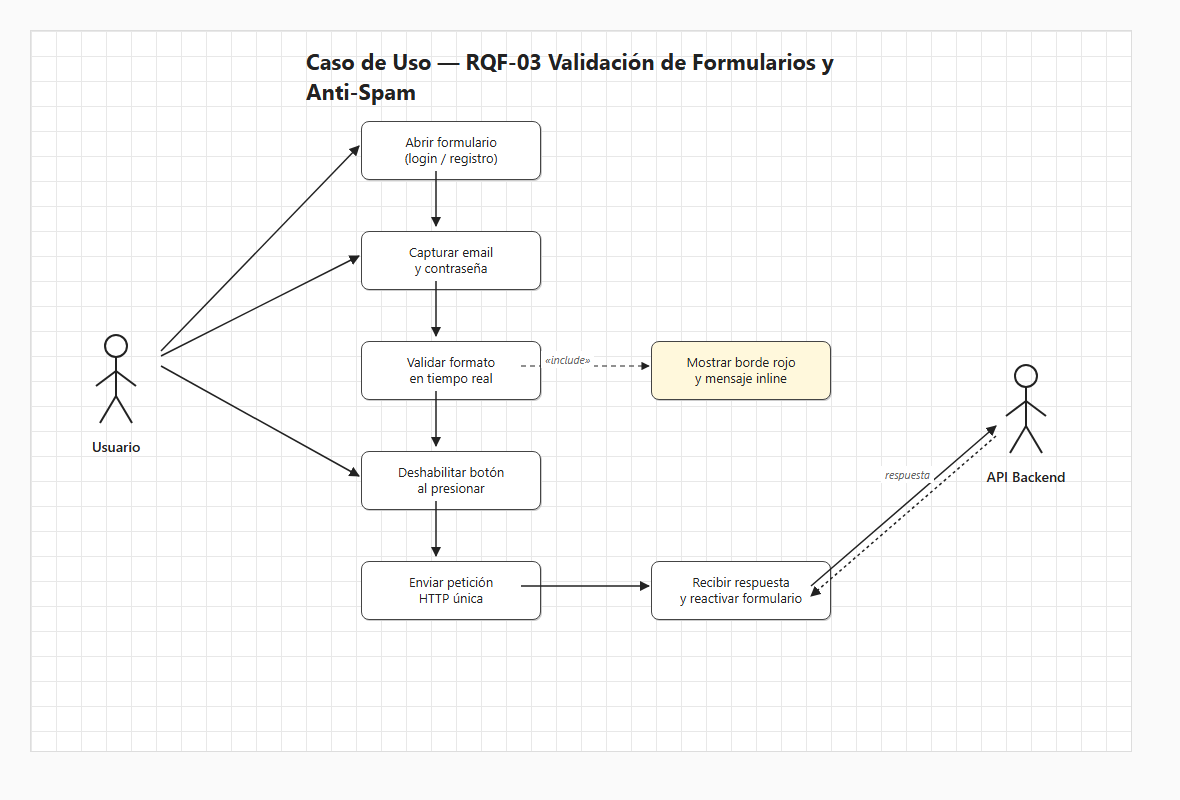
\includegraphics[width=0.85\textwidth]{images/rqf03_validacion.png}
  \caption{Diagrama de casos de uso — Validación de formularios y anti-spam}
\end{figure}

\subsection{RQF-04 — Indicador de conexión y caché offline}

El siguiente diagrama describe el comportamiento del dashboard al detectarse un cambio en la conectividad del dispositivo. El sistema decide entre mostrar datos en vivo, datos cacheados o un banner informativo según el estado de la red.

\begin{figure}[h!]
  \centering
  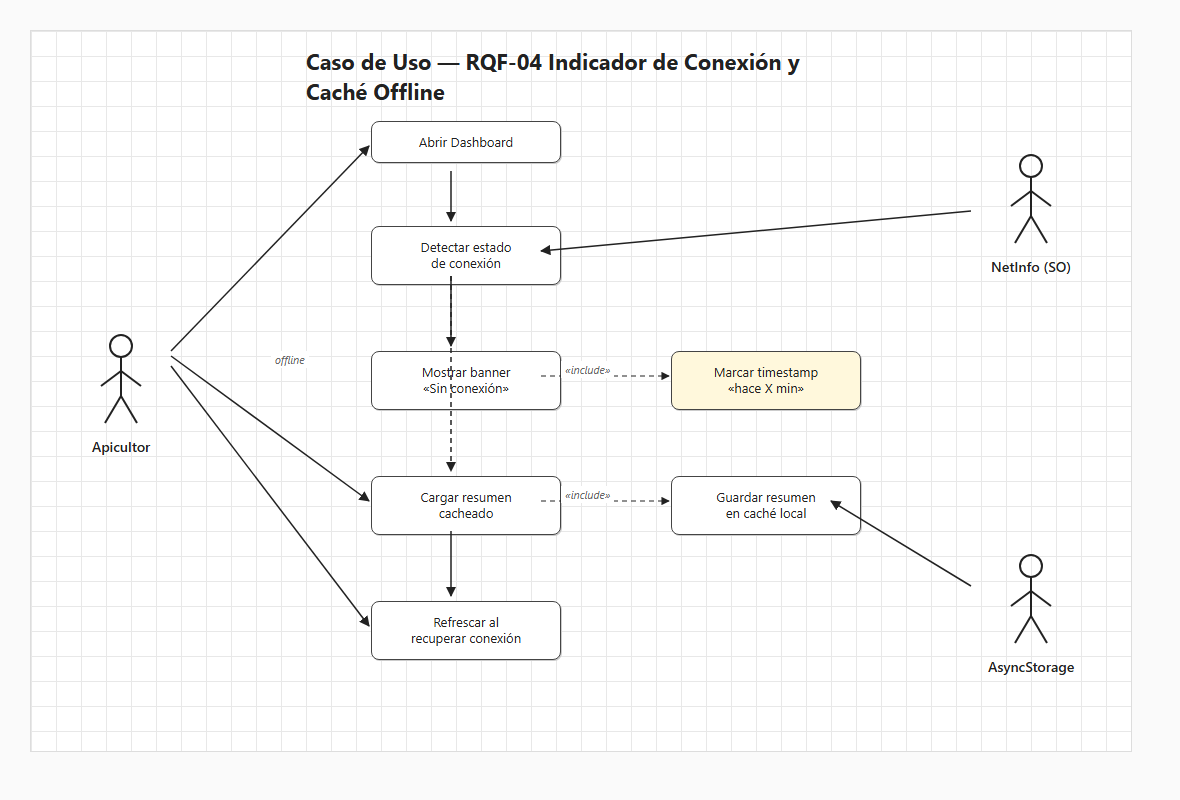
\includegraphics[width=0.85\textwidth]{images/rqf04_offline.png}
  \caption{Diagrama de casos de uso — Indicador de conexión y caché offline}
\end{figure}

\clearpage
\subsection{RQF-05 — Bitácora apícola con calendario}

El siguiente diagrama describe las interacciones del apicultor con la nueva pantalla de bitácora y con el acceso rápido desde la pantalla de detalle de colmena. Ambos puntos de entrada culminan en la persistencia del evento en el backend.

\begin{figure}[h!]
  \centering
  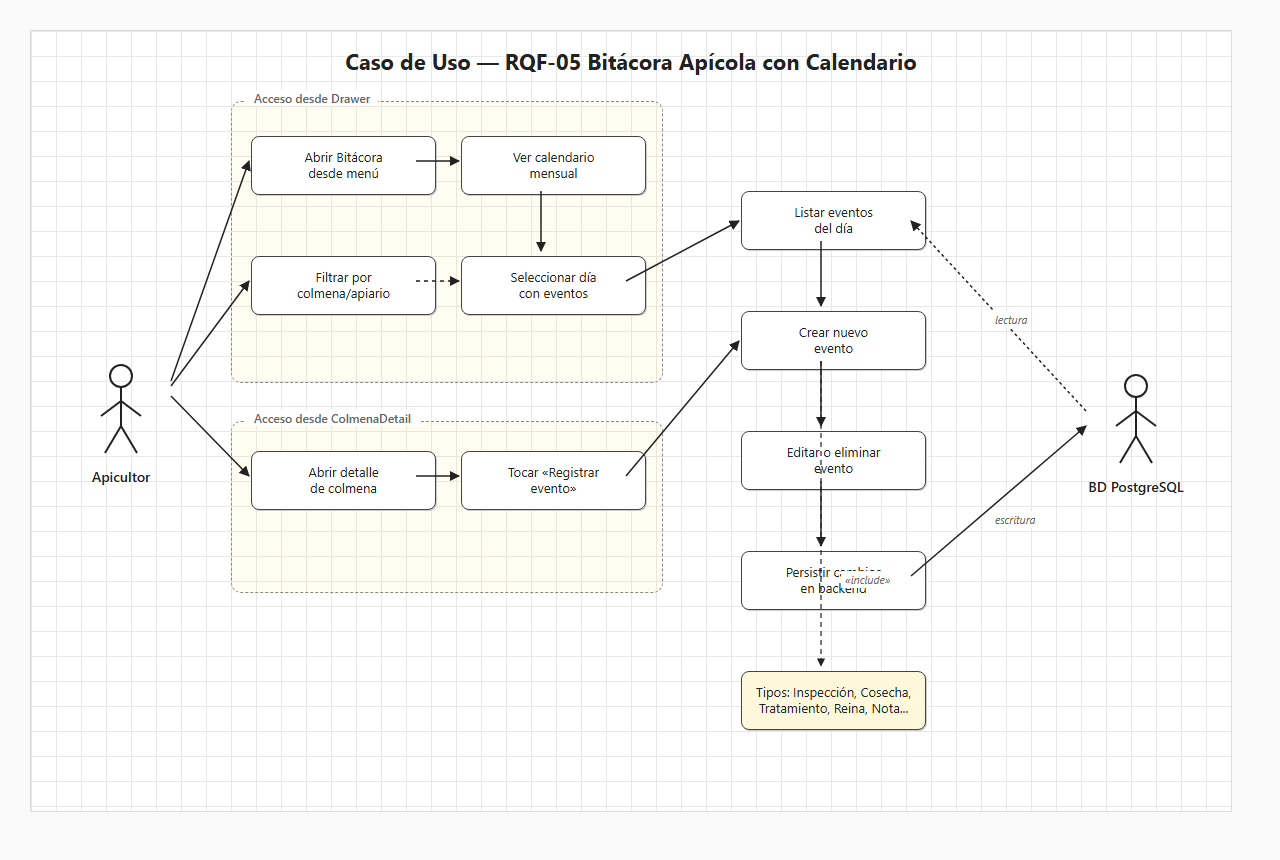
\includegraphics[width=0.95\textwidth]{images/rqf05_bitacora.png}
  \caption{Diagrama de casos de uso — Bitácora apícola con calendario}
\end{figure}

\subsection{Priorización MoSCoW}

\begin{table}[h!]
\centering
\caption{Priorización de los nuevos requerimientos}
\renewcommand{\arraystretch}{1.2}
\begin{tabular}{@{}lp{10cm}@{}}
\toprule
\textbf{Prioridad} & \textbf{Requerimientos} \\
\midrule
\textbf{Must have} & RQF-03 (anti-spam y validación), RQF-04 (caché offline), RNF-03 (bloqueo por inactividad) \\
\textbf{Should have} & RQF-05 (bitácora apícola), RNF-01 (soporte bilingüe), RNF-02 (háptico y toasts) \\
\textbf{Could have} & RNF-04 (compatibilidad multiplataforma validada), RNF-05 (rendimiento $<$ 2s medido y documentado) \\
\textbf{Won't have} & Rediseño visual integral, soporte para wearables/Smart TV e integración con pagos, mapas o IA (fuera del alcance de esta iteración) \\
\bottomrule
\end{tabular}
\end{table}


\end{document}
